\section{硬件部分}
    \subsection{整体设计}
        硬件部分,需要在软件客户端的控制下,产生适当的时钟信号,控制程序运行指定的时钟数或者运行到指定的断点状态。

        运行结束之后,应当将硬件上的信号值发送到客户端,以供调试人员查看信号值,分析芯片运行状况。

        调试工具的硬件部分工作流程如图\ref{process}。

        \begin{figure}[htbp!]
            \centering
            \caption{硬件部分工作流程示意图}\label{process}
            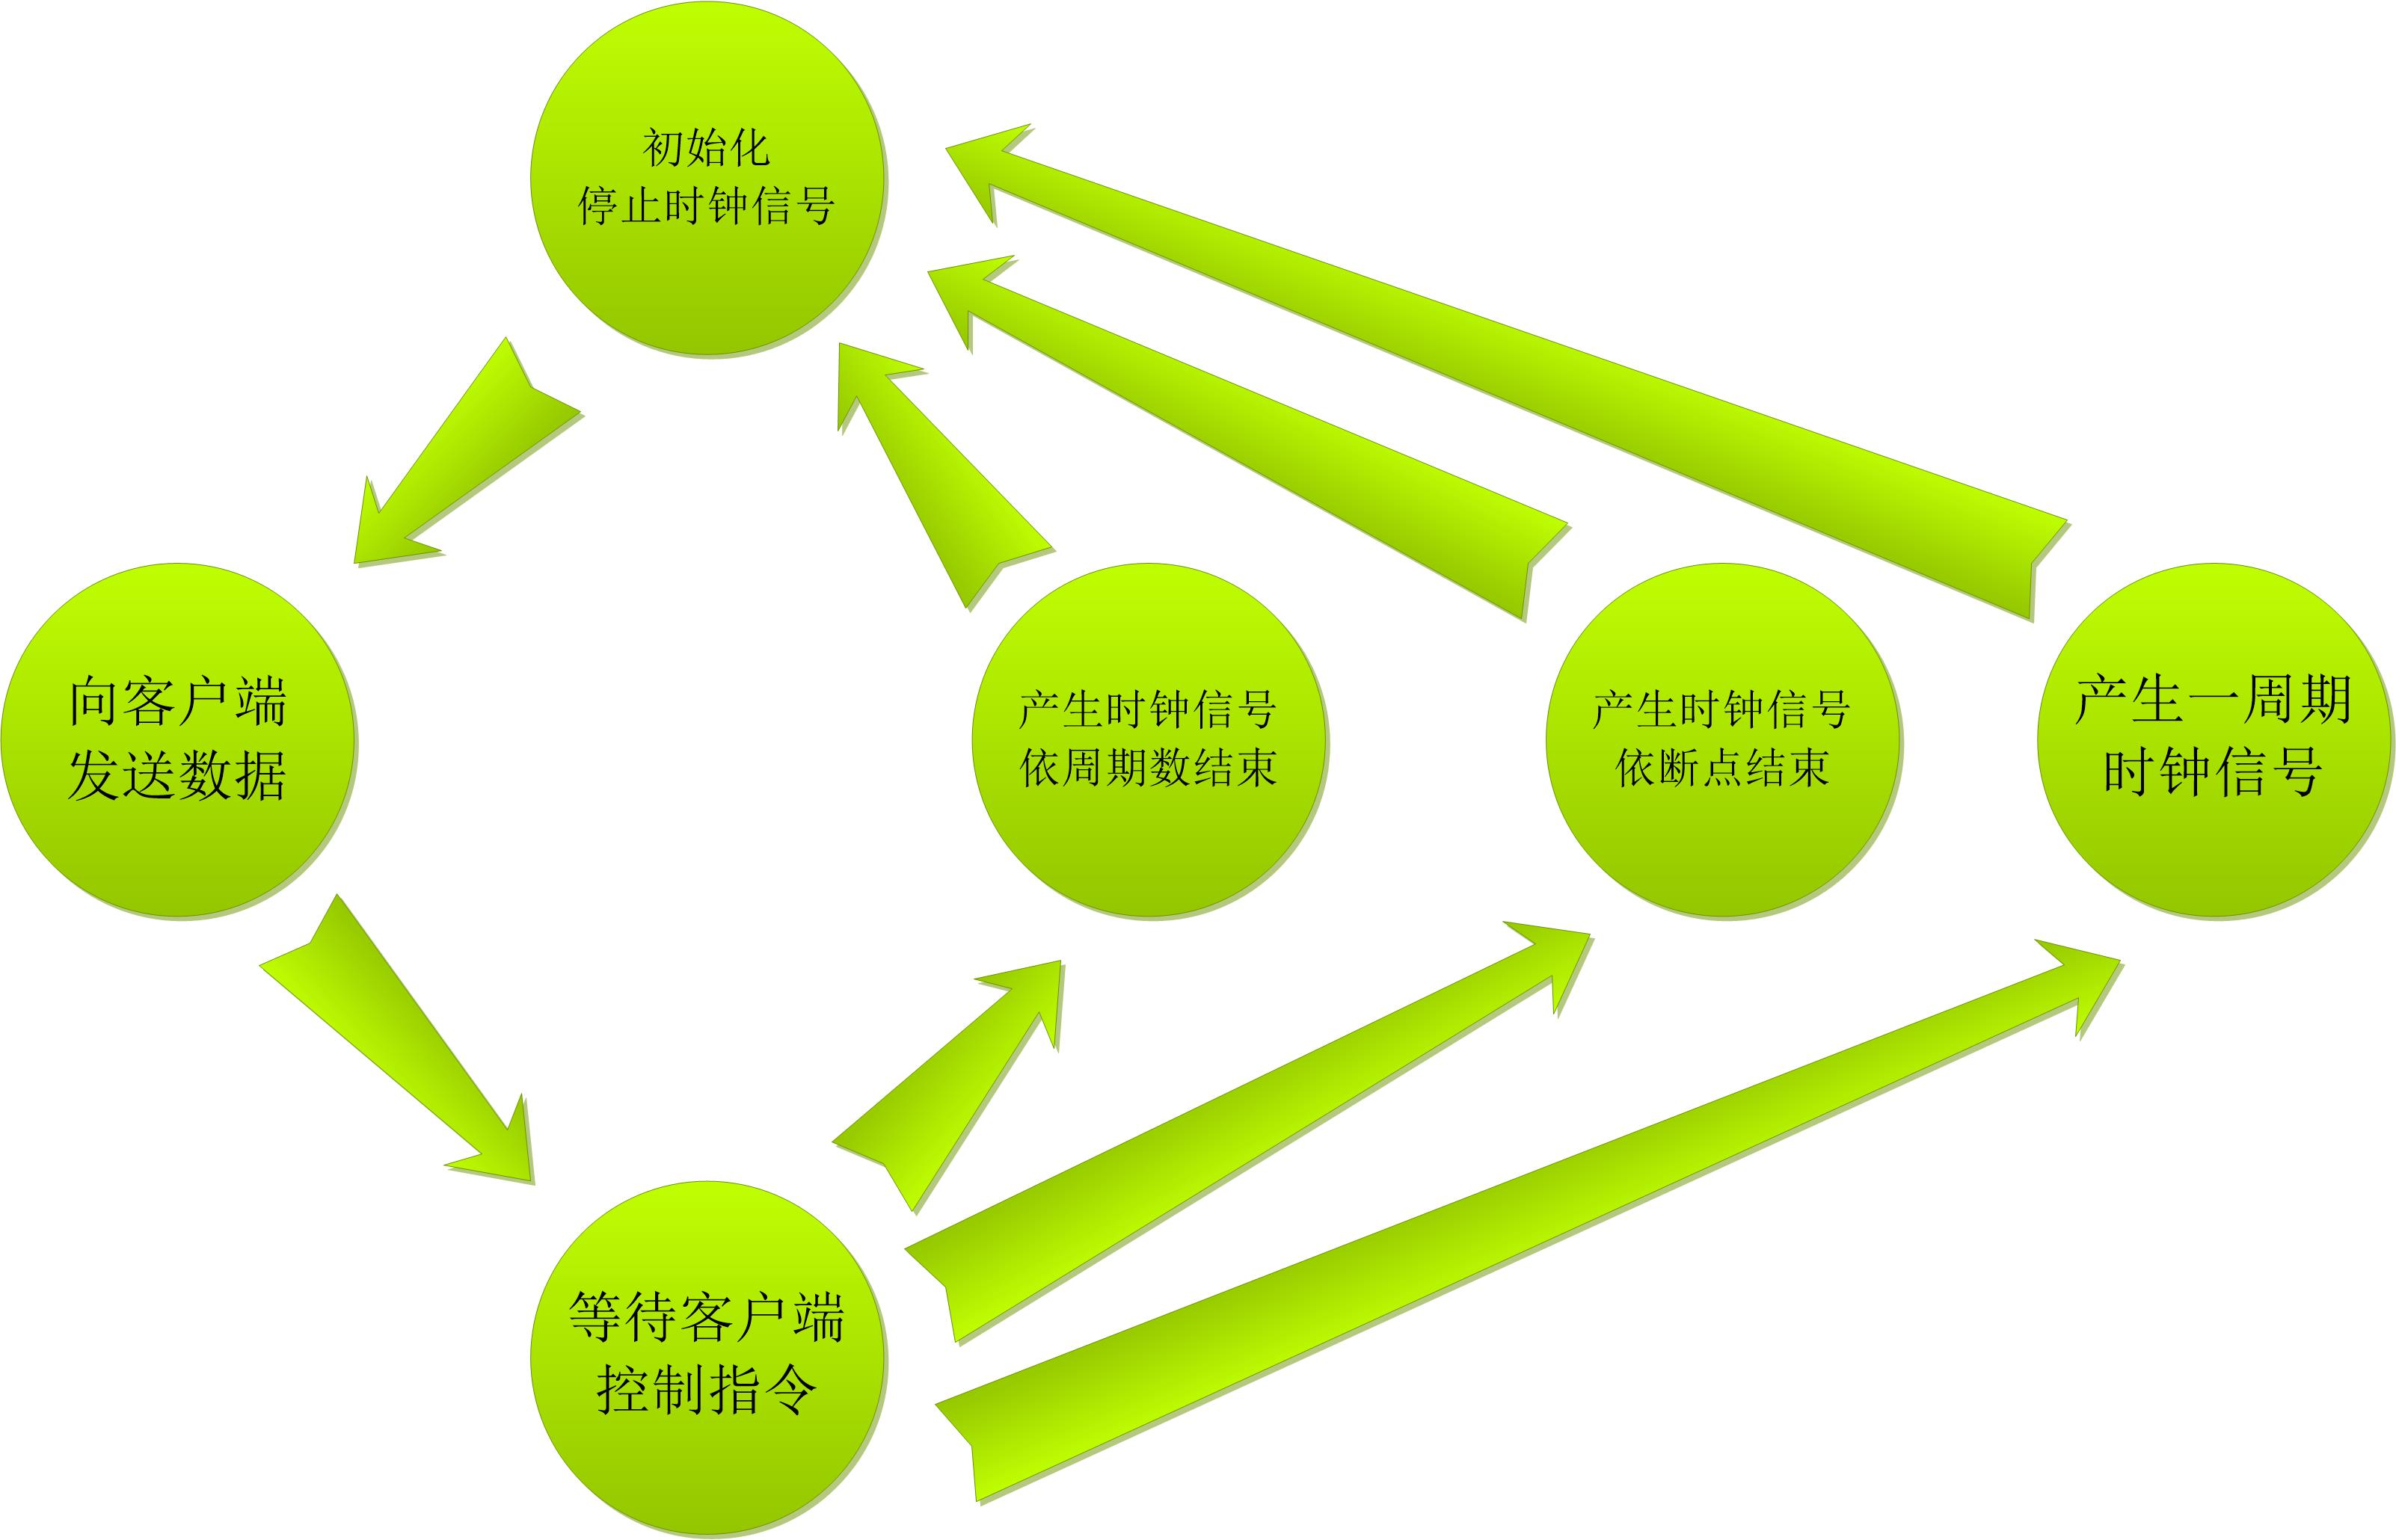
\includegraphics[width=0.5\textwidth]{chart/hardware_path.jpg}
        \end{figure}

        上述功能由两个模块实现,一个模块用于与客户端进行通信,另一个模块用于控制被调试模块的时钟信号以及调试工具的状态跳转。
    \subsection{模块设计}
        \subsubsection{控制模块}
            此模块位于bp\_debug.vhd

            \paragraph{端口说明}
            \mbox{}
                        \begin{tabularx}{\textwidth}{lll}
            \toprule
            端口名          & 端口方向  & 端口类型 \\
            \cmidrule(l){2-3}
            &
            \multicolumn{2}{X}{端口描述} \\
            \midrule
            clk             & in        & std\_logic \\
            \cmidrule(l){2-3}
            &
            \multicolumn{2}{X}{
                时钟输入。
            } \\
            \midrule
            clk\_o             & out        & std\_logic \\
            \cmidrule(l){2-3}
            &
            \multicolumn{2}{X}{
                由此模块产生的时钟信号,可直接作为被测试模块的时钟。
            } \\
            \midrule
            e             & in        & std\_logic \\
            \cmidrule(l){2-3}
            &
            \multicolumn{2}{X}{
                使能信号。
            } \\
            \midrule
            datas             & in        & std\_logic\_vector ( 4095 downto 0 ) \\
            \cmidrule(l){2-3}
            &
            \multicolumn{2}{X}{
                从被测试模块发来的信号值数据。
            } \\
            \midrule
            monitor             & in        & std\_logic\_vector ( 63 downto 0 ) \\
            \cmidrule(l){2-3}
            &
            \multicolumn{2}{X}{
                从被测试模块发来的监控信号数据,用于断点的监控。
            } \\
            \midrule
            serialport\_txd        & out      & std\_logic \\
            \cmidrule(l){2-3}
            &
            \multicolumn{2}{X}{
                串口写端口。
            } \\
            \midrule
            serialport\_rxd             & in        & std\_logic \\
            \cmidrule(l){2-3}
            &
            \multicolumn{2}{X}{
                串口读端口。
            } \\
            \bottomrule
        \end{tabularx}


            \paragraph{内部实现}
            \mbox{}

                控制模块的状态机大致与调试工具硬件部分的工作流程相对应。

                需要查看的信号值部分,从被调试模块获取信号值(默认长度为4096bit),使用组合逻辑的方法根据通信模块给出的字节编号选取对应的字节提供给通信模块。

                调试部分,目前仅支持在上升沿之前断点,实现方式为输出时钟由两个中间值取异或得到。%
                一个中间值的改变由输入时钟下降沿触发,在输出时钟为高电平时对其取反。%
                令一个中间值的改变由输入时钟上升沿触发,在程序运行阶段,且仍需继续运行时,如果输出时钟为低电平,则将其取反。

                被调试模块是否应当继续运行,根据指令的不同而有不同的判断方式。

                对于断点调试而言,当检测信号与段电信号值相同时应当进行停止运行,否则应当继续运行。

                对于继续调试而言,应当无条件给出一个周期的时钟信号,然后按照断点调试判断。

                对于单步调试而言,设置一个倒计时计数器,每次时钟上升沿减一且被调试模块运行,减到0时被调试模块停止运行。

        \subsubsection{通信模块}
            此模块位于com\_debug.vhd

            \paragraph{端口说明}
            \mbox{}

                        \begin{tabularx}{\textwidth}{lll}
            \toprule
            端口名          & 端口方向  & 端口类型 \\
            \cmidrule(l){2-3}
            &
            \multicolumn{2}{X}{端口描述} \\
            \midrule
            clk             & in        & std\_logic \\
            \cmidrule(l){2-3}
            &
            \multicolumn{2}{X}{
                串口发送部分开始信号。
            } \\
            \midrule
            slc             & out        & std\_logic\_vector(15 downto 0) \\
            \cmidrule(l){2-3}
            &
            \multicolumn{2}{X}{
                串口发送的字节编号,用于从上层模块获取对应字节。
            } \\
            \midrule
            data             & in        & std\_logic\_vector ( 7 downto 0 ) \\
            \cmidrule(l){2-3}
            &
            \multicolumn{2}{X}{
                串口发送的字节值,使用编号slc从上层模块获取。
            } \\
            \midrule
            serialport\_txd        & out      & std\_logic \\
            \cmidrule(l){2-3}
            &
            \multicolumn{2}{X}{
                串口写端口。
            } \\
            \midrule
            serialport\_rxd             & in        & std\_logic \\
            \cmidrule(l){2-3}
            &
            \multicolumn{2}{X}{
                串口读端口。
            } \\
            \midrule
            data\_coming             & out        & std\_logic \\
            \cmidrule(l){2-3}
            &
            \multicolumn{2}{X}{
                标志位,表示客户端指令到来。
            } \\
            \midrule
            coming\_data             & out        & std\_logic\_vector ( 135 downto 0 ) \\
            \cmidrule(l){2-3}
            &
            \multicolumn{2}{X}{
                来自客户端的指令信息。
                高64位为客户端第二个参数;
                中64位为客户端第一个参数;
                低8位表示指令类型。
            } \\
            \midrule
            data\_read             & in        & std\_logic \\
            \cmidrule(l){2-3}
            &
            \multicolumn{2}{X}{
                标志位,表示这一指令已经被读取,可以消除指令到来信号。
            } \\
            \bottomrule
        \end{tabularx}


            \paragraph{内部实现}
            \mbox{}

                通信模块包括接受与发送两部分,分别工作,相互不影响,通过软件端、控制模块保证发送与接受的顺序。

                发送部分用于运行结束时,向客户端发送需要的内部信号值。%
                收到控制端的发送开始信号后,从0号字节开始循环发送。%
                这一部分使用slc端口给出字节编号,然后由data读入字节信息,通过串口发送。

                接收部分从软件端接受指令,收到17个字节后,通过标志位通知控制模块数据到来,同时提供数据。%
                收到控制模块读走数据的信号后,接收部分将数据到来标志位清零,同时继续等待新数据到来。

                此部分工作频率默认在50MHz,%
                频率不符会导致此部分不能正常工作。%
                修改频率请在async.v中做修改。

